
\chapter{Vorgehensweise}

\section{Netzarchitektur}

Als Basismodell dient uns das von Nvidia entworfene CNN zur Schätzung eines Steuerbefehls für ein Fahrzeug \cite{nvidia}. Dieses Netz nutzt fünf Faltungsschichten zur Extraktion von Merkmalen mit einer Kerngröße von $(5, 5)$ in den ersten drei Schichten und $(3, 3)$ in den letzten Beiden. Die ersten drei Schichten verwenden außerdem ein Zero-Padding. Darauf folgen drei Dense-Schichten als Regressor.

Unsere Variante dieses Modells nutzt statt der ReLu die ELU als Aktivierungsfunktion. Diese soll den Lernprozess zusätzlich beschleunigen und die Fähigkeit des Netzes zu Generalisieren verbessern \cite{elu}. Zusätzlich haben wir eine L2 Regularisierung für die Gewichte aller Schichten und Dropout jeweils nach den letzten beiden Faltungsschichten hinzugefügt.

In der Vorverarbeitung der Daten wird die Größe der Bilder von $(640, 480, 3)$ (im Format ($H$, $W$, $C$)) auf $(120, 160, 3)$ reduziert und anschließend das obere Drittel des Bildes abgeschnitten, da dies meißt nur Horizont und sonstige Objekte beinhaltet. Die endgültige Größe des Inputs ist dann $(80, 160, 3)$.

Eine Darstellung unseres Netzes mitsamt Vorverarbeitung der Daten ist in \ref{nvidia-model} zu sehen.

\begin{figure}[H]
	\centering
	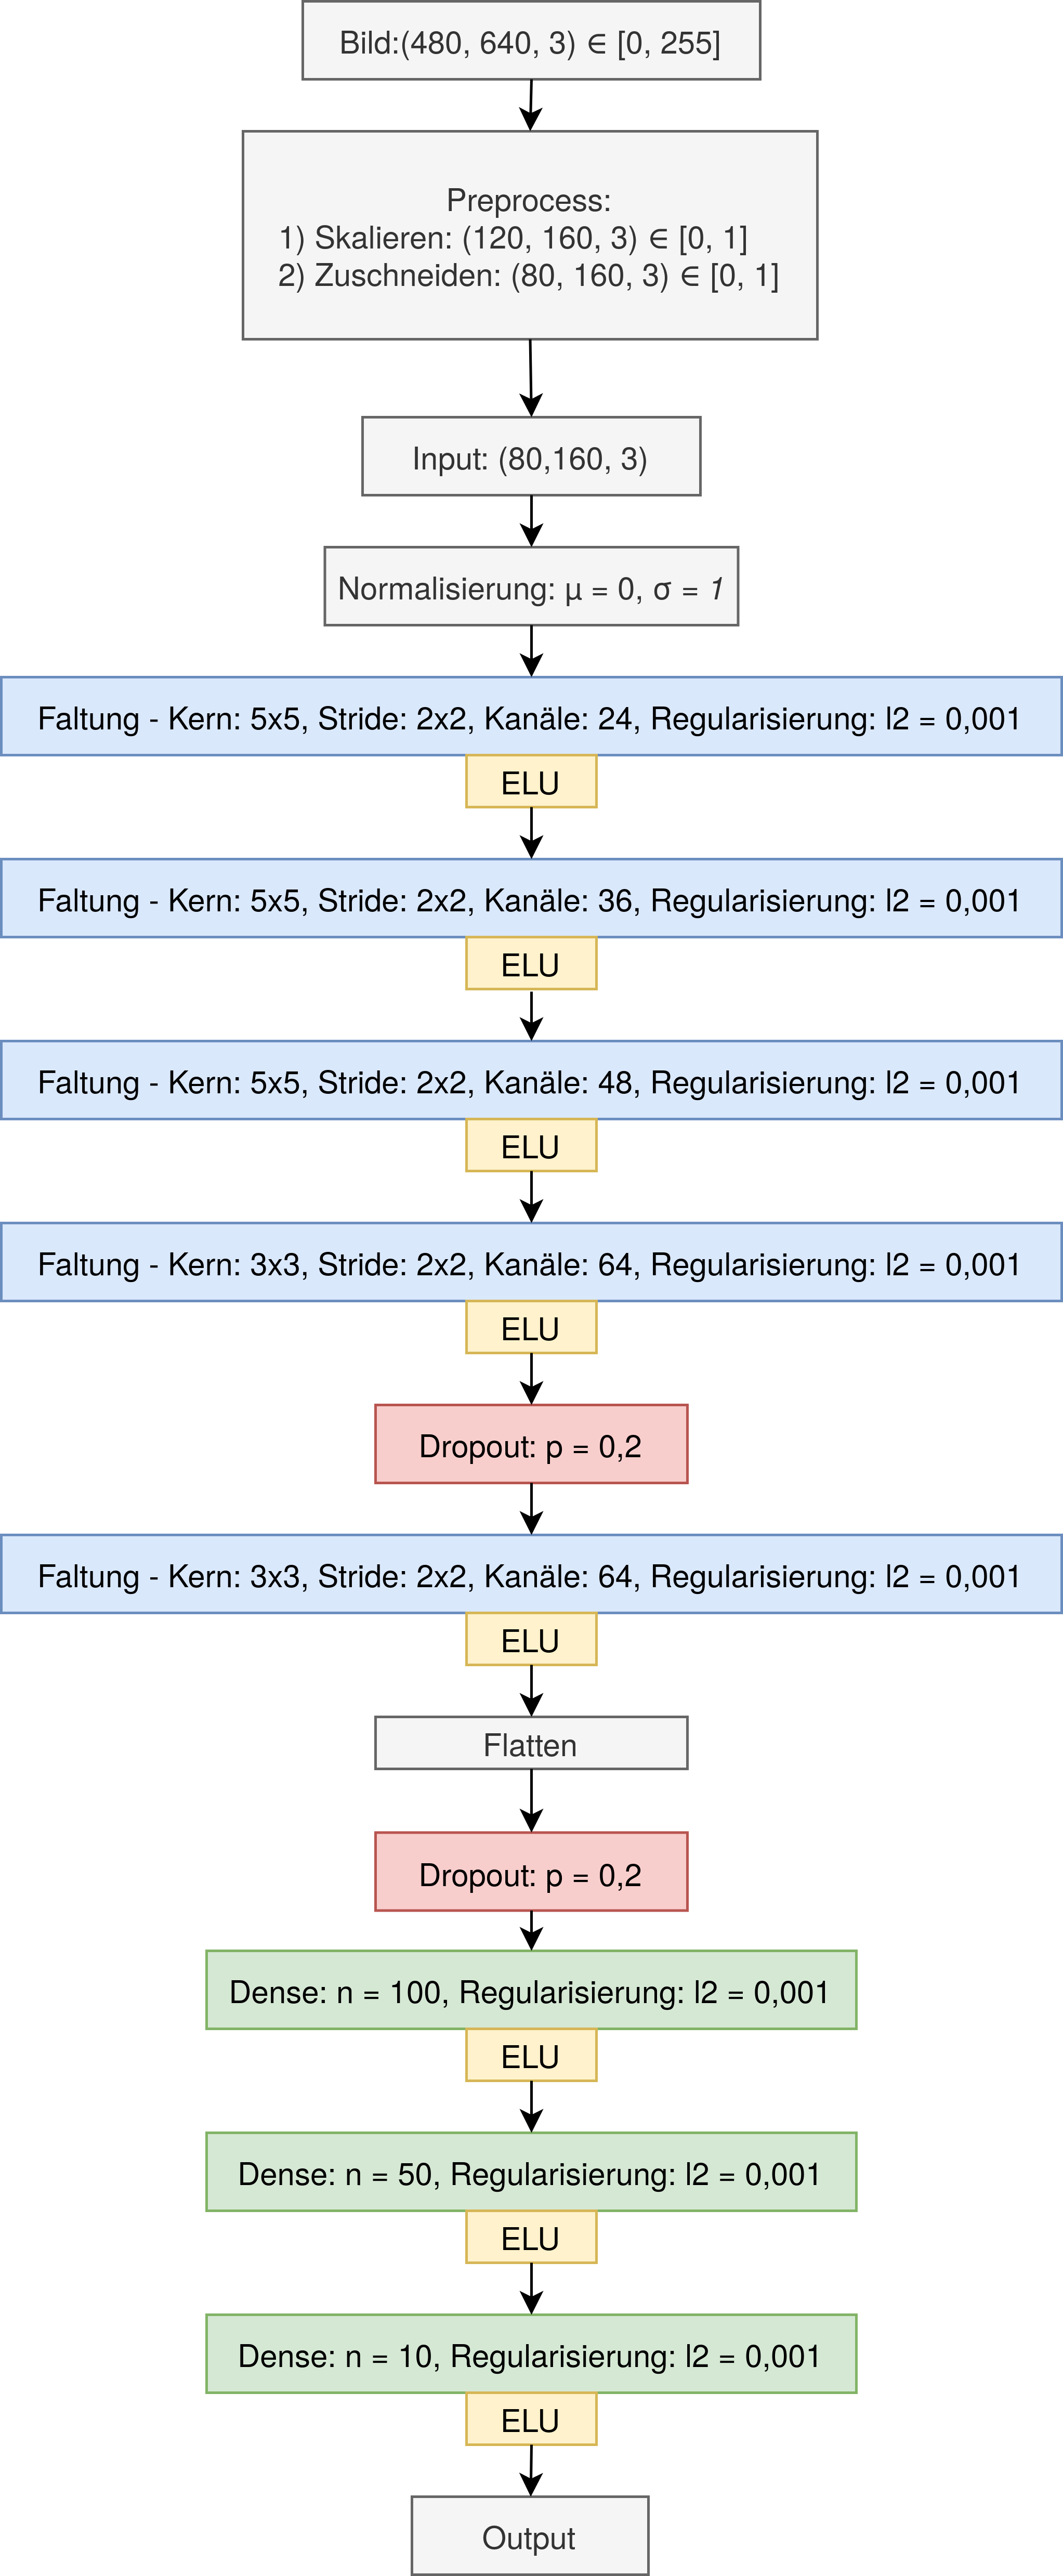
\includegraphics[width=0.65\textwidth]{kapitel4/images/drawio.png}
	\caption{Unsere Variante des Nvidia Modells}
	\label{nvidia-model}
	\vspace{0.2cm}
\end{figure}


\section{Datengewinnung}

Da wir uns in einer simulierten Umgebung befinden, gestaltet sich die Gewinnung von Daten mit entsprechenden Labeln als unproblematisch.
Im Folgenden gehen wir auf zwei Arten möglicher Label und zwei Methoden zur Generierung der Datensätze ein.

\subsection{Label}

Wir verfolgen zwei Ansätze in welchen wir das Netz auf unterschiedliche Ausgaben trainieren. Neben den beiden Werten, auf deren Berechnung im Folgenden eingegangen wird, nutzen wir noch einen dritten Wert als Label, die Art der Kachel auf welcher die Aufnahme entstanden ist.

Im ersten Ansatz ist die Aufgabe des Netzes die Schätzung der Pose des Agenten. Dazu wird vom Simulator eine Aufnahme erzeugt, die Pose des Agenten relativ zur Fahrbahn berechnet und als Label zur Aufnahme abgespeichert. Die Poseninformationen bestehen aus der Distanz zur rechten Fahrbahnmarkierung und der Differenz der Orientierungen von Agent und Tangente der Ideallinie. Mit einem einfachen PD-Regler kann dann ein Steuerbefehl für den Agenten berechnet werden, wobei die Geschwindigkeit fix gewählt wird und die Winkelgeschwindigkeit das Ergebnis des Reglers ist. Da der Distanzwert $d$ von uns als hundertstel Kachelgröße und die Winkeldifferenz in Grad festgelegt wurde, hat eine typische Berechnung folgende Form:\\

\begin{minipage}{\linewidth}
	\begin{lstlisting}[caption={Berechnung eines Steuerbefehls mit PD-Regler}, language=python]
	d, a = environment.cheatmodul.get_lane_pose()
	d_hat_to_center = (d - 20.5) / 100.
	a_hat_in_rad = (a * 2 * np.pi) / 360.
	steering = k_p * d_hat_to_center + k_d * a_hat_in_rad
	speed = 0.2
	observation = environment.step((speed, steering))
	data.append((observation, (d, a)))
	\end{lstlisting}
\end{minipage}

\vspace{.5cm}
Die magische Zahl von 20,5 ist einfach die Verschiebung des Wertes vom rechten Fahrbahnrand zur Mitte der Fahrspur, so dass das Ergebnis als Fehler zum Soll (also null) interpretiert werden kann. Das Teilen durch hundert ergibt dann einen Wert in Kachelgrößen, statt hundertstel Kachelgröße.
Zur Vollständigkeit ist im Code noch stark vereinfacht verdeutlicht, wie Aufnahme und zugehöriges Label zustande kommen und gespeichert werden.

Das Schätzen der Pose hat den Vorteil, dass die Informationen anderweitig verwendet werden könnten, beispielsweise zur Lokalisierung des Agenten in einem Monte-Carlo Verfahren.\\

Im zweiten Ansatz trainieren wir das Netz direkt auf entsprechende Steuerbefehle in der Form Geschwindigkeit und Winkelgeschwindigkeit $(v, \omega)$. Dazu benutzen wir ein einfaches Expertensystem, welches mehr Informationen in die Berechnung des Befehls miteinbezieht, als nur die relative Pose des Agenten zum aktuellen Zeitpunkt. Dabei wird ein in einer definierten Distanz voraus liegender Punkt auf der Ideallinie gesucht. Befindet sich dieser Punkt in einer Kurve, oder sind die Orientierungen von Agent und Tangente der Fahrspur zu verschieden, wird $v$ als die Hälfte einer Referenz-Geschwindigkeit festgelegt. Bei Geraden ist $v$ die volle Referenz-Geschwindigkeit. Die Winkelgeschwindigkeit $\omega$ ist das Skalarprodukt aus dem Vektor, welcher von Roboter in Richtung voraus liegenden Punkt zeigt und dem Einheitsvektor, welcher vom Agenten aus nach rechts zeigt.

\begin{minipage}{\linewidth}
	\begin{lstlisting}[caption={Berechnung eines Steuerbefehls mit einfachem Expertensystem}, language=python]
	
	projected_angle, closest_point, curve_point = environment._get_projected_angle_difference(lookup_distance)
	tile = environment.get_tile(curve_point)
	if 'curve' in tile['kind'] or abs(projected_angle) < 0.92:
		v *= 0.5
	point_vec = curve_point - environment.cur_pos
	point_vec /= np.linalg.norm(point_vec)
	right_vec = np.array([math.sin(self.env.cur_angle), 0, math.cos(self.env.cur_angle)])
	omega = np.dot(right_vec, point_vec)
	
	\end{lstlisting}
\end{minipage}

\subsection{Observationen}

Bei der Gernerierung der Datensätze verfolgen wir ebenfalls zwei Ansätze. Im ersten, naiven Ansatz lassen wir den Agenten selbstständig durch die Umgebung fahren, wobei für jeden Aufruf der \texttt{step()} Methode eine Aufnahme mit entsprechendem Label gespeichert wird. Die Verteilung der Werte sollte demnach jener entsprechen, welche der Agent beim selbstständigen Fahren tatsächlich erlebt.

Im zweiten Ansatz lassen wir den Agenten nur eine gewisse Anzahl von Schritten, also \texttt{step()} Aufrufen, fahren und rufen dann die \texttt{reset()} Methode des Simulators auf, welche den Agenten an eine zufällige, aber valide Pose zurücksetzt. Valide bedeutet, dass die Position befahrbar und frei von Kollisionen mit anderen Objekten ist.
Der Gedanke dahinter ist, dass so die Verteilung der Werte mehr ``Ausnahmefälle'' beinhaltet. Denn sollte das Netz nicht im Stande sein, die Spur ähnlich gut halten zu können wie der PD-Regler oder das Expertensystem, wird es oft in Situationen geraten, auf welche es nicht trainiert wurde. Die Werteverteilung sollte so ähnlich sein zu dem, was der Agent erlebt, falls er öfters ``crashen'' sollte.

\subsection{Datensätze}

Wie erleutert, ergeben sich zwei Ansätze zur Zusammensetzung des Labels und zwei Ansätze um die Verteilung der Labels zu beeinflussen. Insgesamt ergeben sich vier Datensätze. Die zwei PD-Datensätze ``PD'' und ``PD-Rand'' und zwei Experten-Datensätze, ``Expert'' und ``Expert-Rand''. Der Zusatz ``Rand'' steht dabei für den höheren Anteil an Zufallsposen.\\

\begin{figure}[H]
	\centering
	\begin{subfigure}{0.5\textwidth}
		\centering
		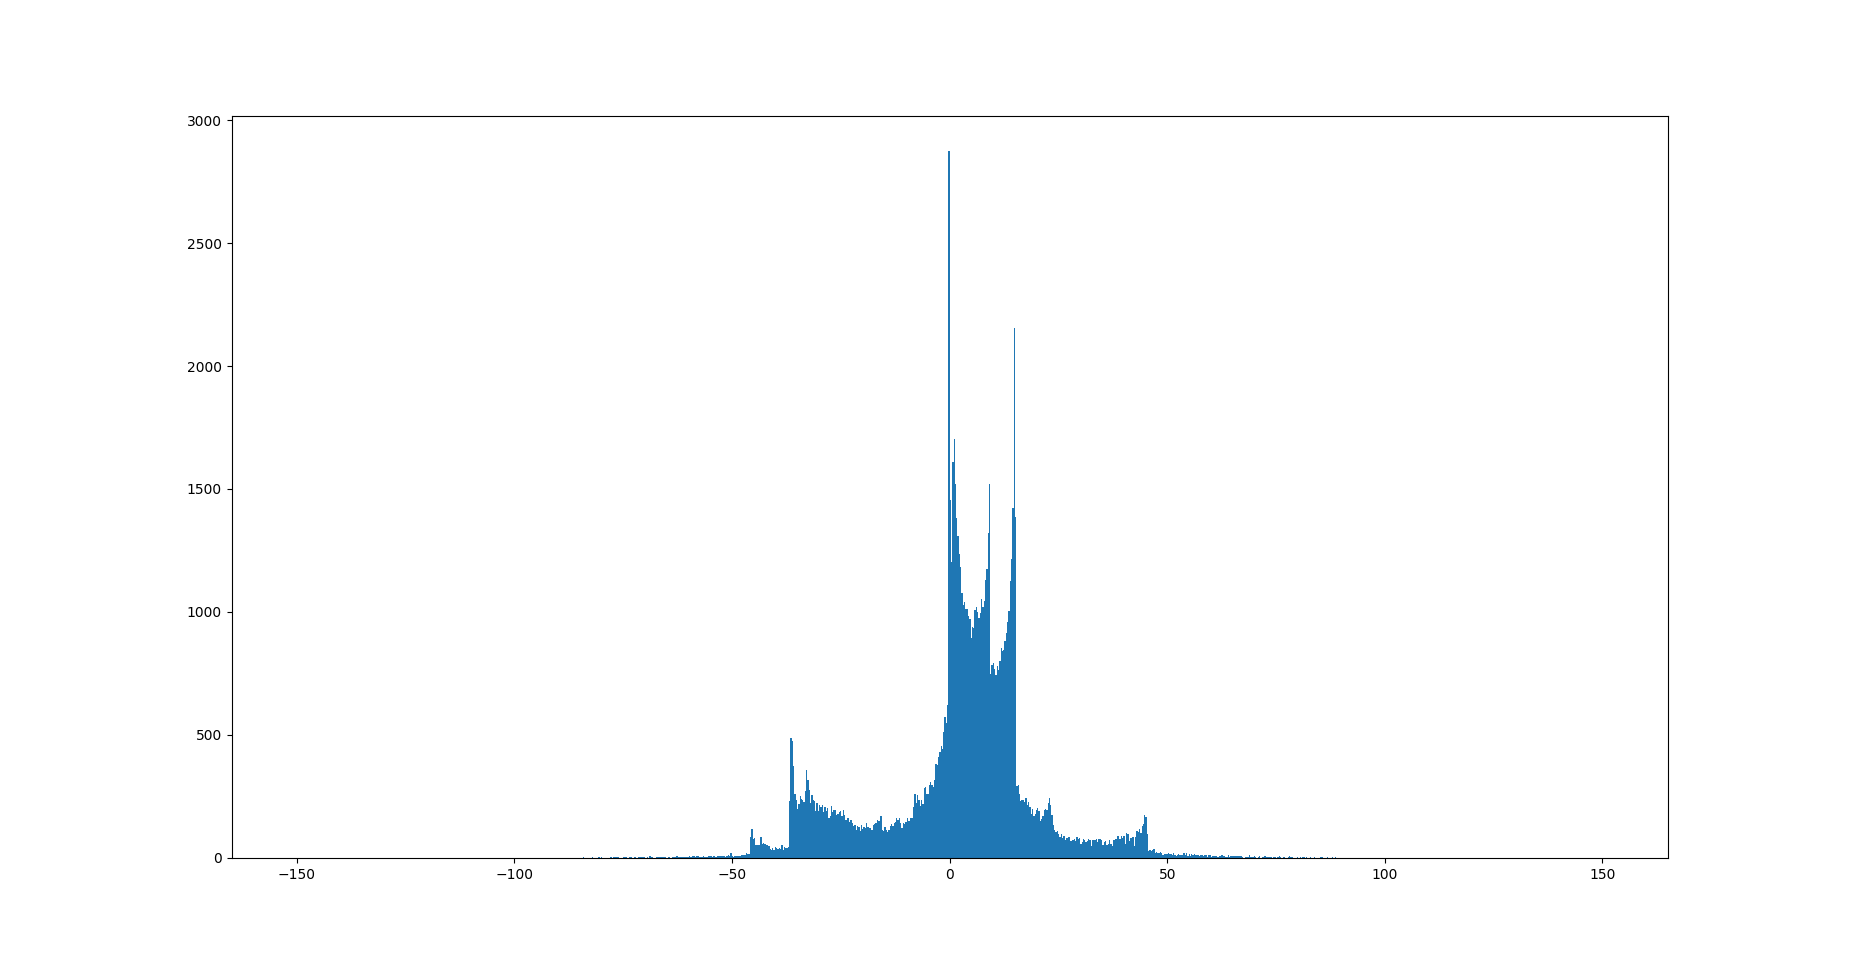
\includegraphics[width=\linewidth]{kapitel4/images/plots/pd/pd-angles.png}
		\caption{Winkel des PD Datensatzes}
		\label{pd-drive-angles}
	\end{subfigure}%
	\begin{subfigure}{0.5\textwidth}
		\centering
		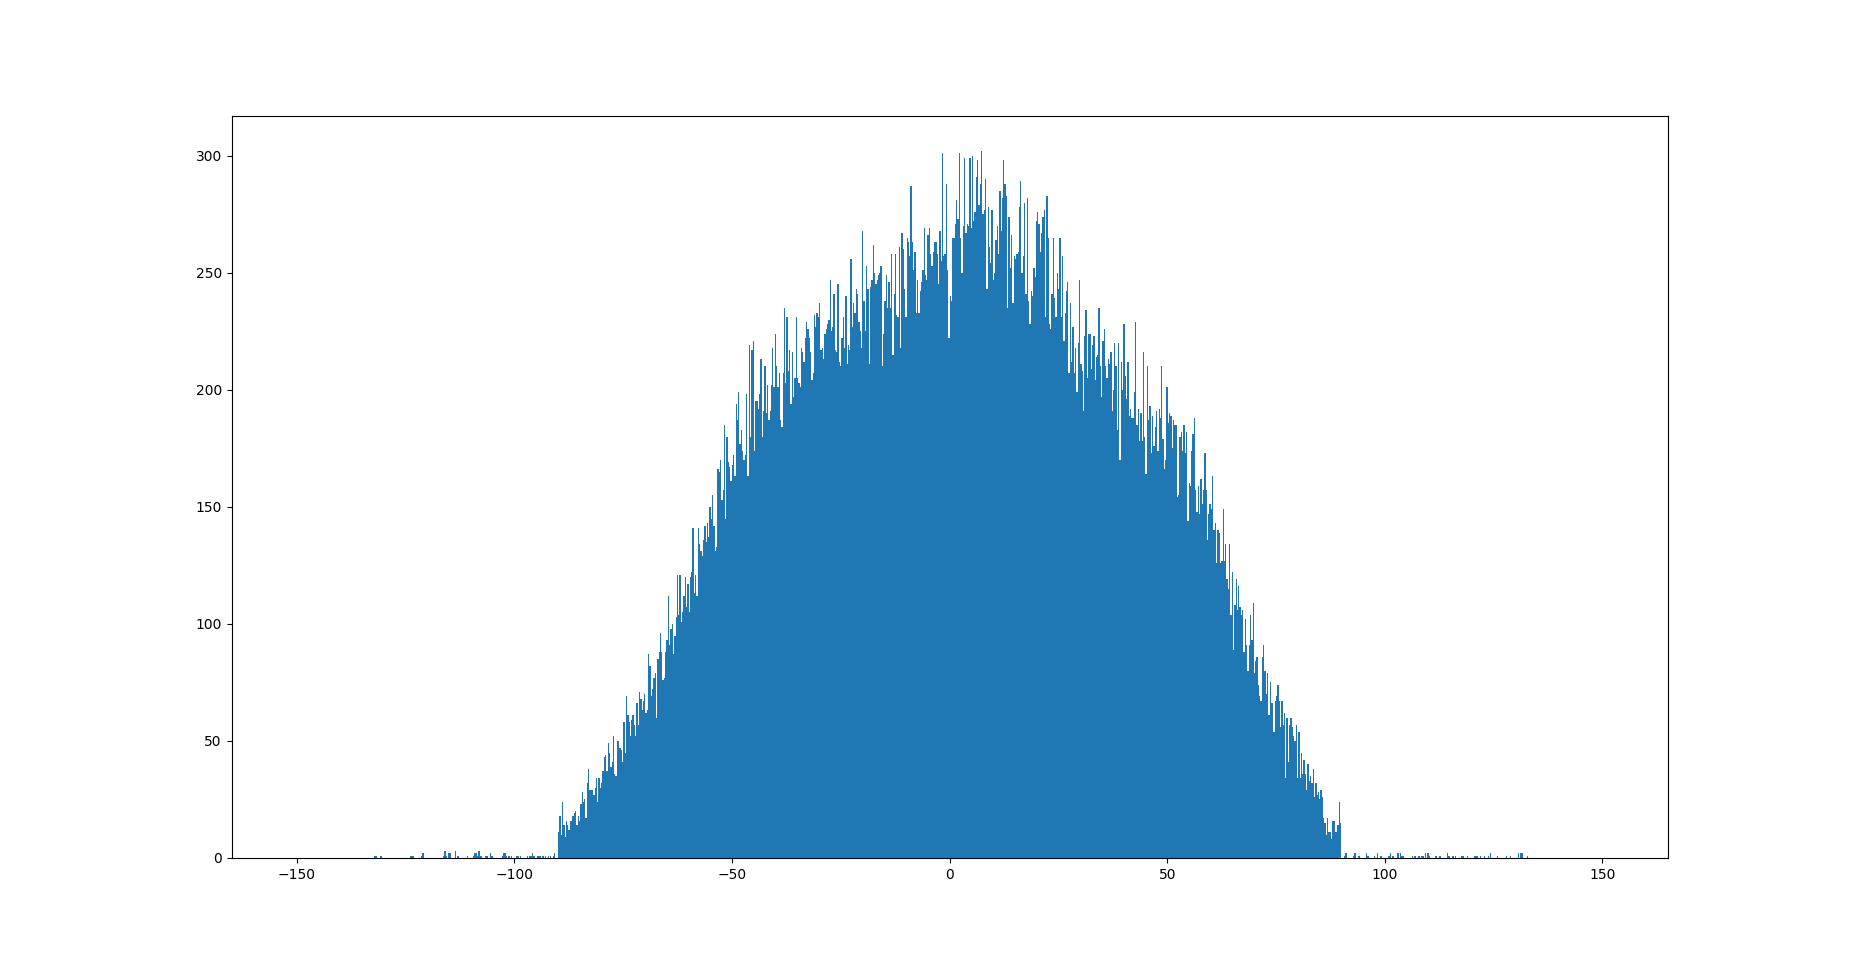
\includegraphics[width=\linewidth]{kapitel4/images/plots/pd-rand/pd-rand-angles.png}
		\caption{Winkel des PD-Rand Datensatzes}
		\label{pd-rand-angles}
	\end{subfigure}
	\caption{Verteilungen der Winkel der PD Datensätze}
	\label{pd-angles}
\end{figure}


\begin{figure}[H]
	\centering
	\begin{subfigure}[h]{0.5\textwidth}
		\centering
		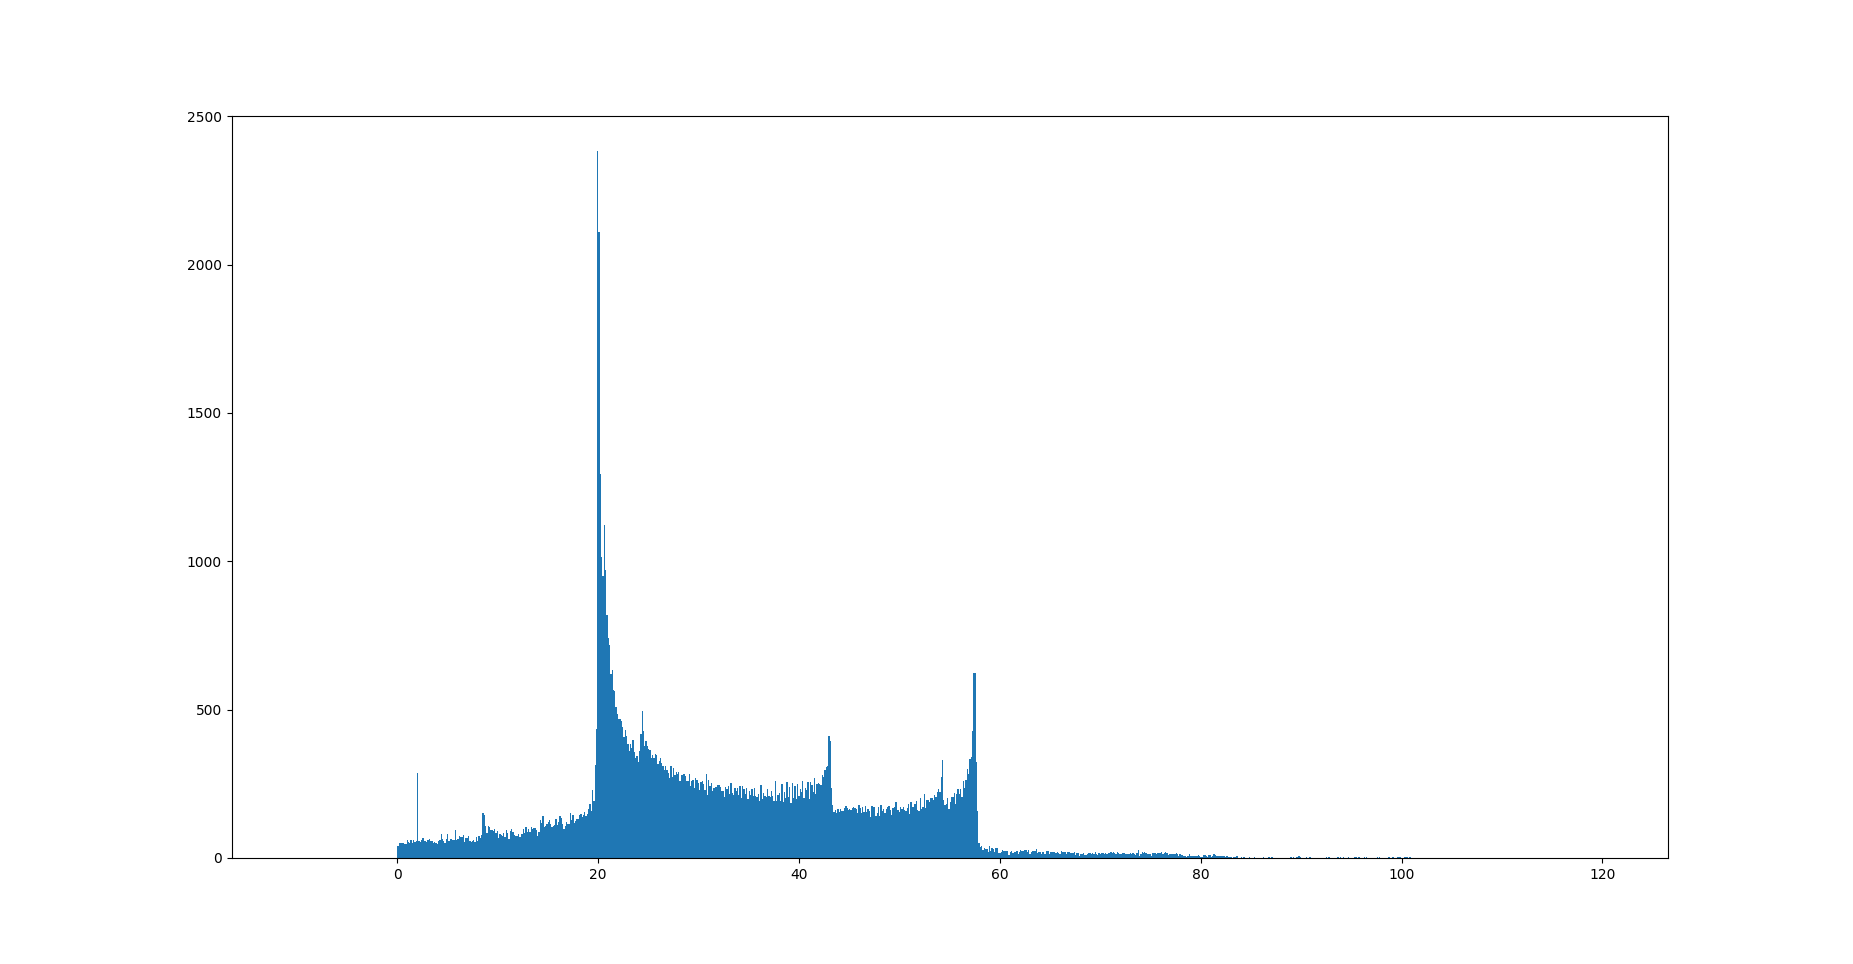
\includegraphics[width=\linewidth]{kapitel4/images/plots/pd/pd-distances.png}
		\caption{Entfernungswerte des PD Datensatzes}
		\label{pd-drive-distances}
	\end{subfigure}%
	\begin{subfigure}[h]{0.5\textwidth}
		\centering
		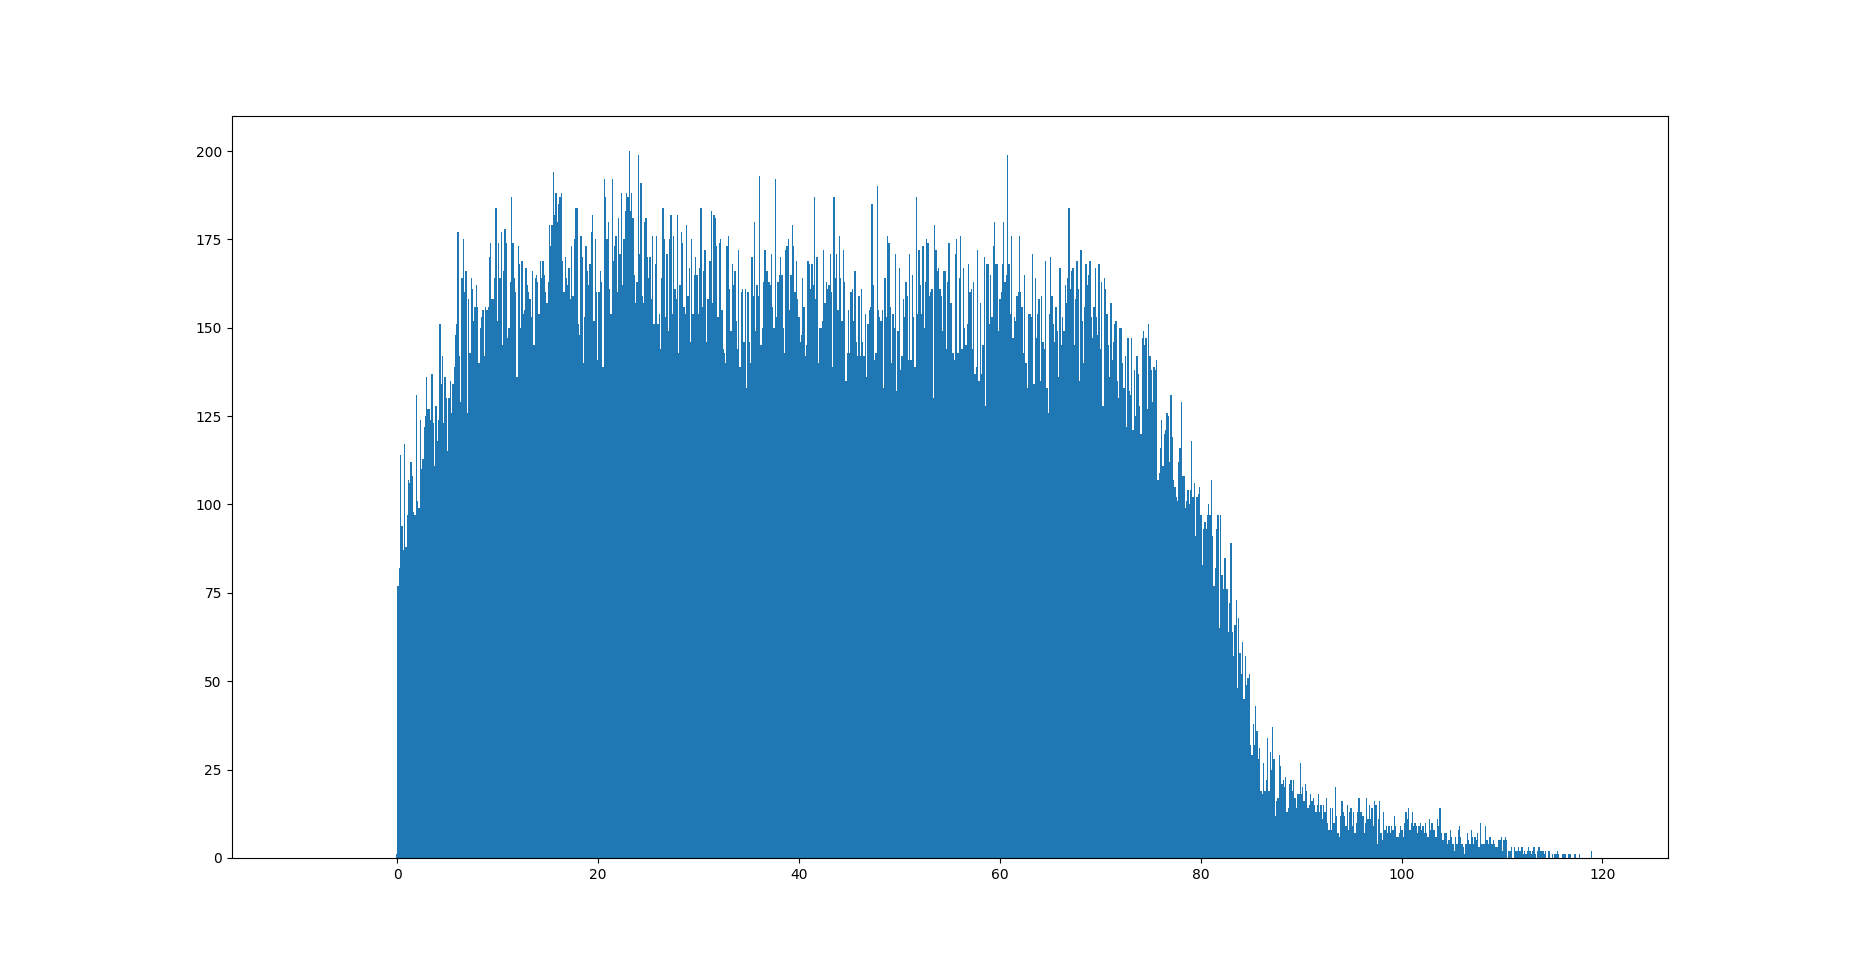
\includegraphics[width=\linewidth]{kapitel4/images/plots/pd-rand/pd-rand-distances.png}
		\caption{Entfernungswerte des PD-Rand Datensatzes}
		\label{pd-rand-distances}
	\end{subfigure}
	\caption{Verteilungen der Entfernungswerte der PD Datensätze}
	\label{pd-distances}
\end{figure}

Wie in \ref{pd-angles} und \ref{pd-distances} erkennbar, ist die Verteilung von sowohl Entfernungswerten, als auch Winkeldifferenzen im  ``PD-Rand'' Datensatz wesentlich gleichmäßiger als im ``PD''-Datensatz.


\begin{figure}[H]
	\centering
	\begin{tabular}[t]{|l|l|}
		\hline
		\textbf{Datensatz} & \textbf{Größe} \\
		\hline
		PD & 100.000 \\
		\hline
		PD-Rand & 100.000 \\
		\hline
		Expert & 100.000 \\
		\hline
		Expert-Rand & 100.000 \\
		\hline
	\end{tabular}
	\caption{Größe der erzeugten vier Datensätze}
\end{figure}

\begin{figure}[H]
	\centering
	\begin{subfigure}{0.5\textwidth}
		\centering
		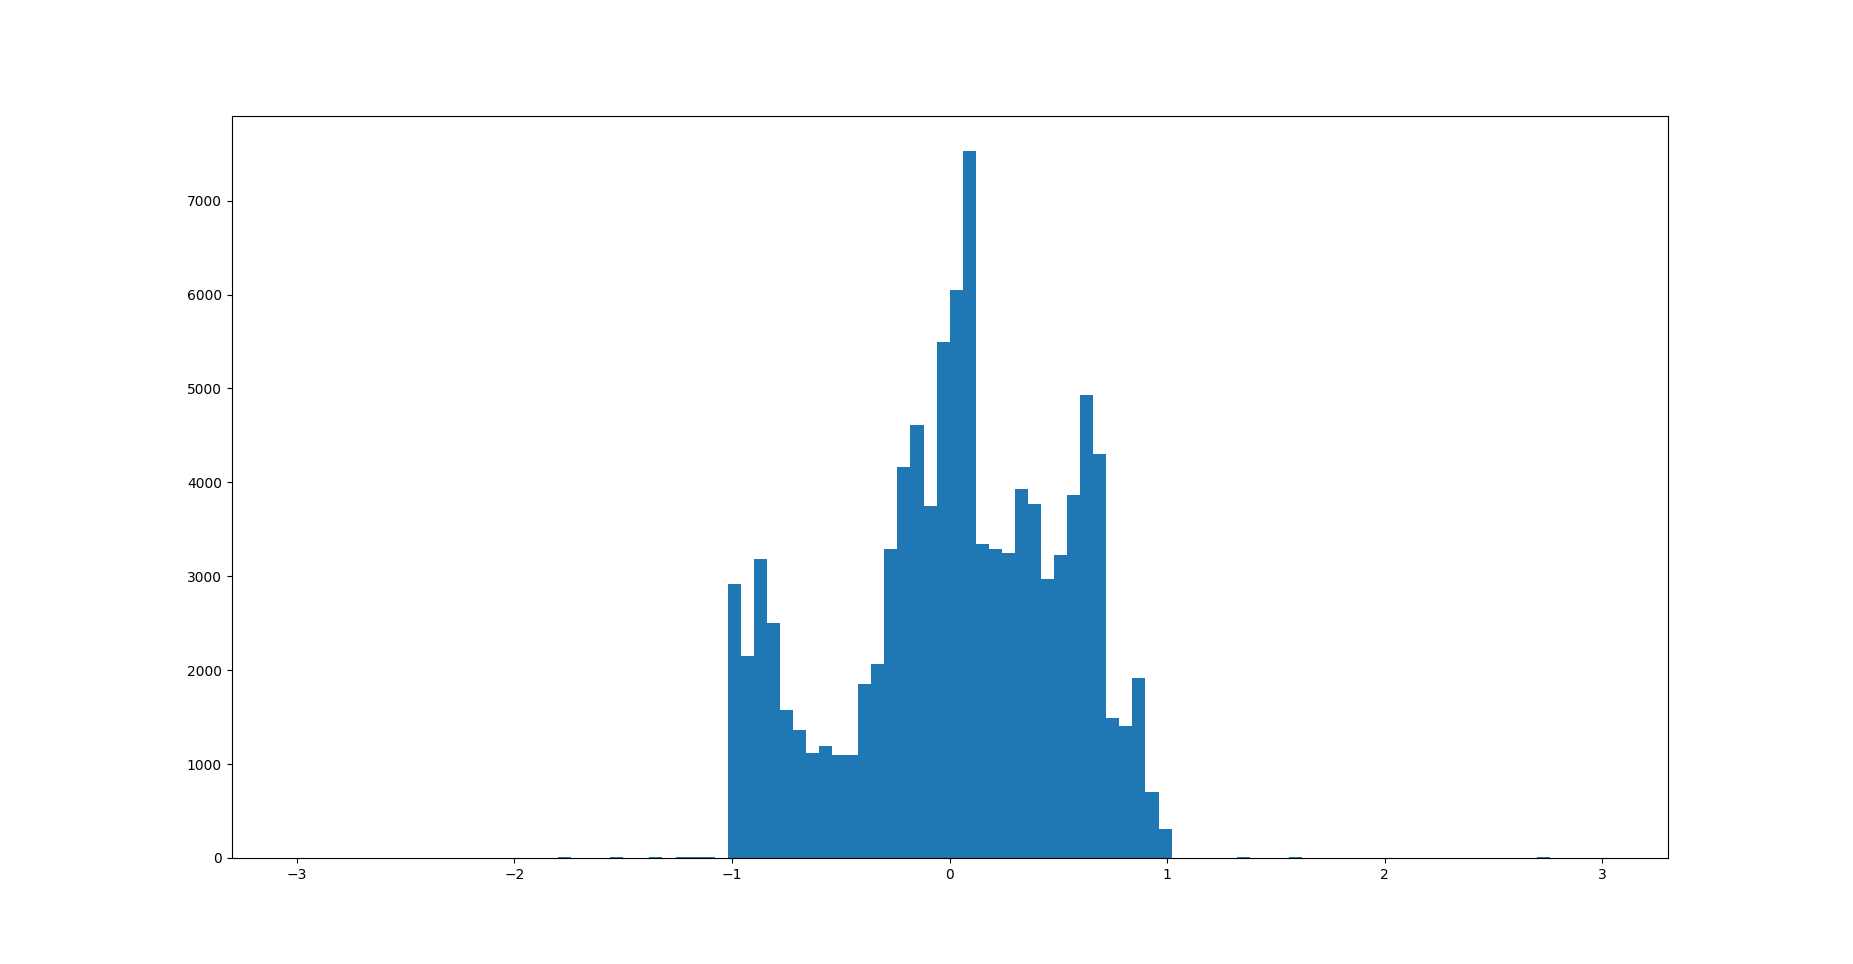
\includegraphics[width=\linewidth]{kapitel4/images/plots/expert/expert-angular_velocities.png}
		\caption{Winkelgeschwindigkeiten des Expert Datensatzes}
		\label{expert-angular}
	\end{subfigure}%
	\begin{subfigure}{0.5\textwidth}
		\centering
		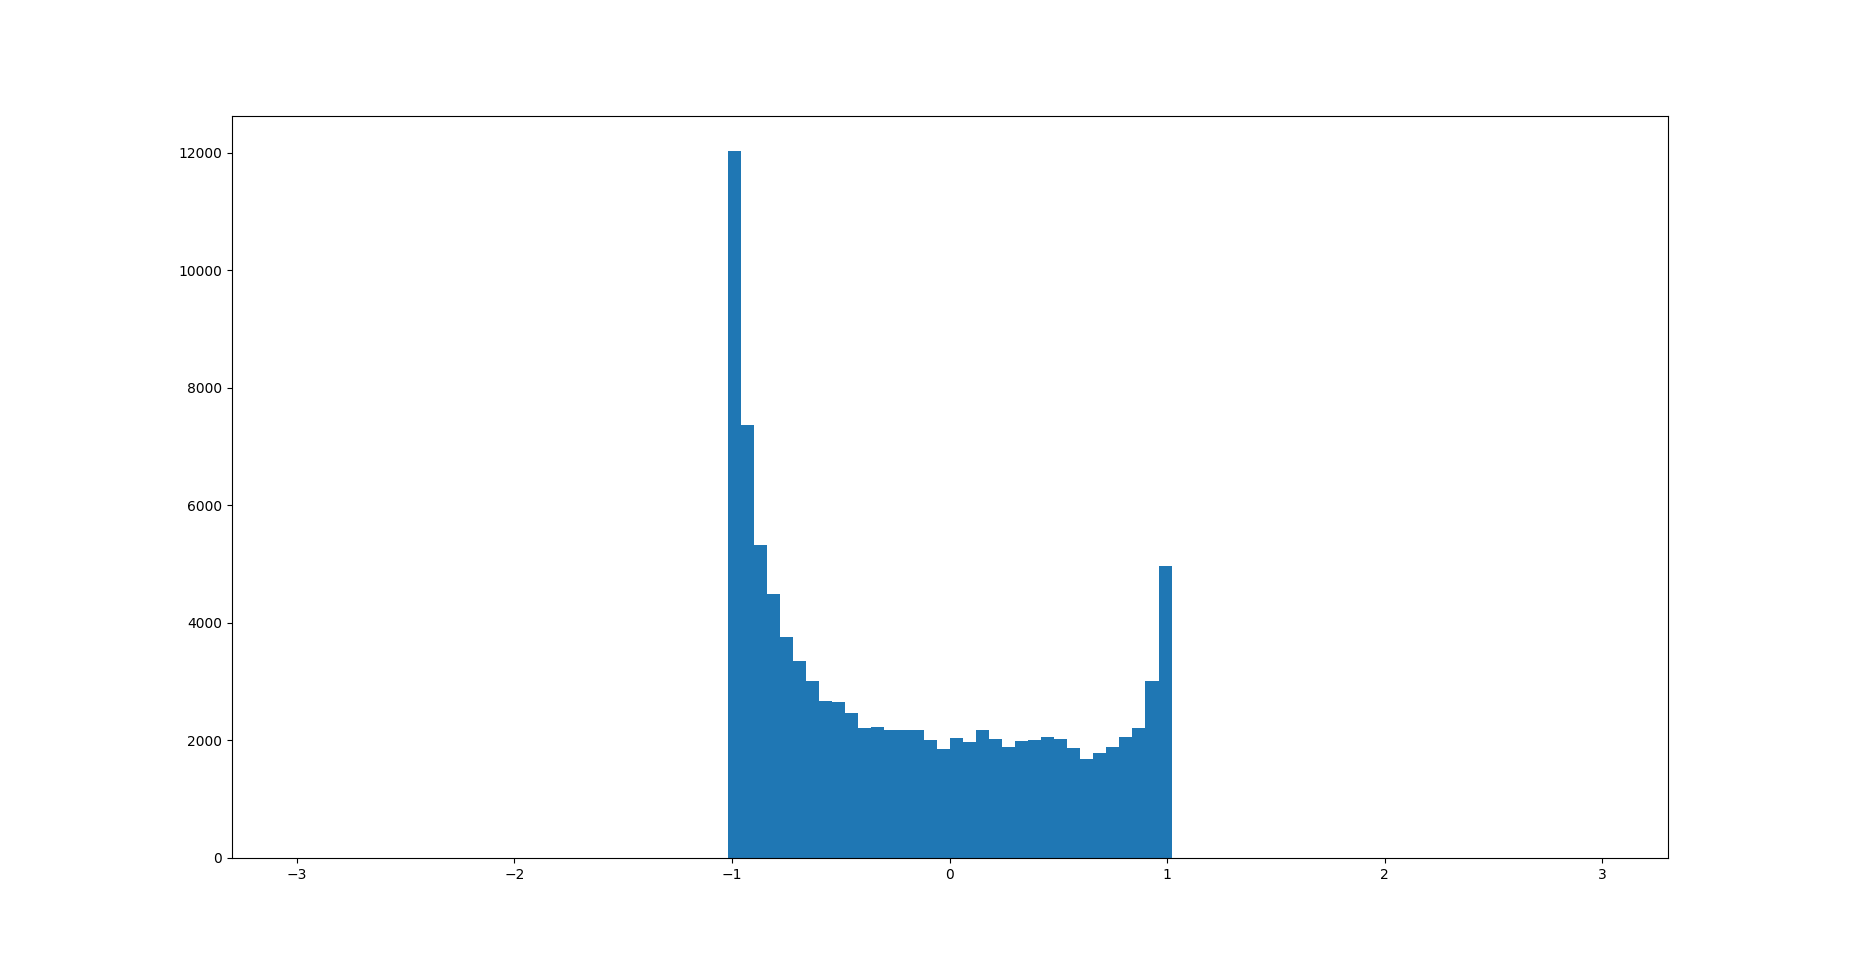
\includegraphics[width=\linewidth]{kapitel4/images/plots/expert-rand/expert-random-angular_velocities.png}
		\caption{Winkelgeschwindigkeiten des Expert-Rand Datensatzes}
		\label{expert-rand-angular}
	\end{subfigure}
	\caption{Verteilungen der Winkelgeschwindigkeiten der Expert Datensätze}
	\label{expert-angles}
\end{figure}


In den Expertendatensätzen \ref{expert-angles} lässt sich ebenfalls ein deutlicher Unterschied in der Verteilung der berechneten Winkelgeschwindigkeiten des Steuerbefehls feststellen. In \ref{expert-rand-angular} ist eine Menge an Maximalwerten von -1 und 1 erkennbar (der Wertebereich durch das Skalarprodukt, kann zum Beispiel mit Faktor $\pi$ multipliziert werden).
Auf die berechneten Geschwindigkeiten der Expertendatensätze muss nicht eingegangen werden, da zum einen aufgrund unseres einfachen Expertensystems die Verteilung nur aus zwei Werten besteht und zum Anderen sich diese Verteilung durch die Ansätze nicht wesentlich unterscheidet.\\


\section{Lernprozess}

Das Feintuning des Modells und die Wahl der Hyperparameter wurden in einem langwierigen Prozess experimentell erarbeitet.\\


\begin{center}
	\begin{tabular}[t]{|l|l|}
		\hline
		Lerngeschwindigkeit & 0.0002 \\
		\hline
		Batch Größe & 32 \\
		\hline
		Optimizer & Adam \\
		\hline
		Anzahl Epochen & 50 \\
		\hline
		Verlustfunktion & MSE \\
		\hline
	\end{tabular}
\end{center}


Wir setzen den Adam Optimizer ein, da dieser durch adaptive Lernraten oft einen schnelleren Lernprozess ermöglicht und generell in der Literatur oft zum Einsatz kommt. Wir parametrisieren Adam mit einer initialen Lernrate von $0.0002$. Diese ergab in Kombination mit einer Batchgröße von 32 in den meißten Fällen eine gute Konvergenz.

Die Größe der Batch von 32 soll einen Kompromiss bilden zwischen Geschwindigkeit des Prozesses und der Fähigkeit des Netzes zu Generalisieren. Eine Batchgröße über 32 hat sich bereits als unvorteilhaft erwiesen \cite{keskar2017largebatch}.

Als Fehlerfunktion wären prinzipiell sowohl MSE als auch MAE vorstellbar. Eine l2 Fehlerfunktion hat den Vorteil, dass Ausreißer in den Daten durch das Quadrat in der Funktion härter bestraft werden. Aber obwohl unsere Daten nur wenige Ausreißer aufweisen, hat sich in Experimenten die MAE nicht deutlich von der MSE unterschieden. Da MSE in der Literatur häufiger zum Einsatz kommt, blieben wir mit unserer Wahl bei ihr.

Den Prozess ließen wir mit einer Dauer von 50 Epochen laufen.  Häufig ist schon nach wenigen Epochen erkennbar, ob die Kombination an gewählten Parametern eine gute Konvergenz ergibt. Aber sollte die Konfiguration konvergieren, geben 50 Durchläufe genug Zeit ein Minimum zu finden.
